\section{张量分解初步：CP、Tucker 与 SVD 的关系}
\label{sec:03-Linear-Algebra/09-Tensors/02}

一份电商日志摊成三阶数组：一万个用户、一千件商品、五十二周，五亿多个数。你想把它压小，顺便看看里面有几条主要机制。

矩阵时代的做法轮廓清楚。跑 SVD，截到前 \(R\) 项，Eckart--Young 保证这是所有秩不超过 \(R\) 的矩阵里离原矩阵最近的一个，误差等于被砍掉的奇异值的平方和开根号，见\hyperref[sec:03-Linear-Algebra/07-SVD-and-Data-Applications/03]{``低秩近似：用少数方向保留主要结构''}。换台机器再跑一遍，结果一样。

三阶的现场是另一副样子。用同一份数据、同一个秩 \(R\) 跑两次 CP 分解，只把随机初始化换掉，得到的因子对不上，重构误差也不同。第一反应多半是怀疑实现有 bug。实现没有问题——高阶把矩阵世界里几件被当成理所当然的事一起收走了。

这一节把两条从矩阵出发的思路各推一遍：``照着 SVD 多加几个向量''给出 CP 分解，``先在每个模找一个低维子空间，再记下子空间之间怎么交互''给出 Tucker 分解。沿途标出哪些保证还在，哪些没了。

\subsection{CP 把立方体写成秩一立方体之和}

上一节的秩一项 \(a_r\otimes b_r\otimes c_r\) 分量为 \((a_r)_i(b_r)_j(c_r)_k\)。CP 分解（CANDECOMP/PARAFAC）尝试

\[
\mathcal X\approx\sum_{r=1}^{R}a_r\otimes b_r\otimes c_r ,
\]

能精确写出的最少项数称为 CP 秩。把各项的向量按列收进因子矩阵 \(A,B,C\)，第 \(r\) 个成分就在三个模上各给一条模式：一组用户偏好、一组商品属性、一条时间强度曲线，相乘得到一个可分离的立方体；若干个这样的立方体叠加，表达若干条潜在机制的共存。

\begin{center}
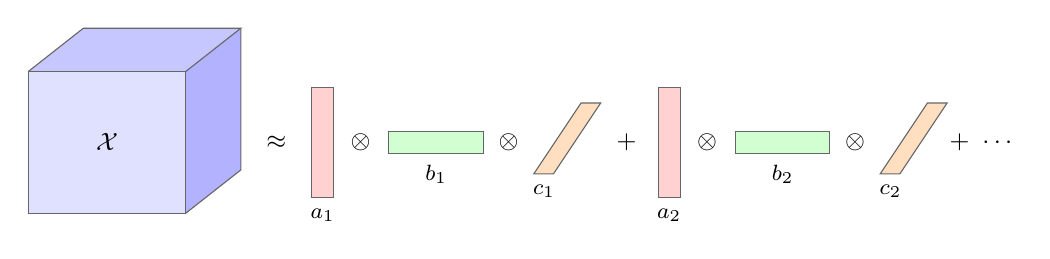
\begin{tikzpicture}[x=1cm,y=1cm,font=\small,>=stealth]
  \fill[blue!12] (0,0) -- (2.0,0) -- (2.0,-1.8) -- (0,-1.8) -- cycle;
  \fill[blue!22] (0,0) -- (2.0,0) -- (2.7,0.55) -- (0.7,0.55) -- cycle;
  \fill[blue!30] (2.0,0) -- (2.7,0.55) -- (2.7,-1.25) -- (2.0,-1.8) -- cycle;
  \draw[black!60] (0,0) -- (2.0,0) -- (2.0,-1.8) -- (0,-1.8) -- cycle;
  \draw[black!60] (0,0) -- (0.7,0.55) -- (2.7,0.55) -- (2.0,0);
  \draw[black!60] (2.7,0.55) -- (2.7,-1.25) -- (2.0,-1.8);
  \node at (1.0,-0.9) {\(\mathcal X\)};
  \node at (3.15,-0.9) {\(\approx\)};
  \begin{scope}[shift={(3.6,0)}]
    \draw[black!60,fill=red!18] (0,-0.2) rectangle (0.28,-1.6);
    \node[below,font=\footnotesize] at (0.14,-1.62) {\(a_1\)};
    \node at (0.62,-0.9) {\(\otimes\)};
    \draw[black!60,fill=green!18] (0.98,-0.76) rectangle (2.18,-1.04);
    \node[below,font=\footnotesize] at (1.58,-1.06) {\(b_1\)};
    \node at (2.5,-0.9) {\(\otimes\)};
    \draw[black!60,fill=orange!25] (2.82,-1.3) -- (3.07,-1.3) -- (3.67,-0.4) -- (3.42,-0.4) -- cycle;
    \node[below,font=\footnotesize] at (2.95,-1.32) {\(c_1\)};
  \end{scope}
  \node at (7.6,-0.9) {\(+\)};
  \begin{scope}[shift={(8.0,0)}]
    \draw[black!60,fill=red!18] (0,-0.2) rectangle (0.28,-1.6);
    \node[below,font=\footnotesize] at (0.14,-1.62) {\(a_2\)};
    \node at (0.62,-0.9) {\(\otimes\)};
    \draw[black!60,fill=green!18] (0.98,-0.76) rectangle (2.18,-1.04);
    \node[below,font=\footnotesize] at (1.58,-1.06) {\(b_2\)};
    \node at (2.5,-0.9) {\(\otimes\)};
    \draw[black!60,fill=orange!25] (2.82,-1.3) -- (3.07,-1.3) -- (3.67,-0.4) -- (3.42,-0.4) -- cycle;
    \node[below,font=\footnotesize] at (2.95,-1.32) {\(c_2\)};
  \end{scope}
  \node at (12.1,-0.9) {\(+\ \cdots\)};
\end{tikzpicture}

\emph{CP 把立方体拆成若干个秩一立方体，每一项在三个模上各出一个向量。存储从 \(IJK\) 个数降到大约 \(R(I+J+K)\) 个，压缩全靠 \(R\) 小；为了压低重构误差不断加大 \(R\)，表示可能比原数据还贵。}
\end{center}

这套算术在工程上就是压缩本身。把一层卷积核当成四阶张量做 CP 或 Tucker 近似，参数和乘加次数一起下降，推理提速；多路观测数据（用户\(\times\)商品\(\times\)时间、被试\(\times\)脑区\(\times\)频段）里，成分则被当成可解释的机制读。两种用法对分解的要求并不相同：前者只在乎重构误差和算子开销，后者还要求因子稳定、可重复、换个初始化不变样。

\subsection{SVD 是二阶时的一次幸运合流}

矩阵秩一项 \(\sigma_ru_rv_r^{\trans}\) 可以把 \(\sigma_r\) 吸进任一向量，写成 \(a_r\otimes b_r\)。所以矩阵的秩分解就是二阶 CP。SVD 在此之上额外选出左右两组正交因子，并把尺度集中成一列非负、降序的奇异值。

矩阵里，非零奇异值个数、列空间维数、最少秩一项数是同一个数的三种说法。到了三阶，这三种说法分家：CP 秩只继承``最少秩一外积项数''这一条，别的各走各路。后果相当具体。实三阶张量的 CP 秩可以超过任何一个模的维数，\(\min(I,J,K)\) 不再是上界；同一尺寸下典型秩还可能不止一个，随机取一个 \(2\times2\times2\) 实张量，落在秩 2 与秩 3 上的概率都为正。行秩等于列秩那种整齐，在这里没有对应物。

另外两样奢侈品也一并交出。高阶 CP 一般不能要求三个模的因子同时正交，也没有一列可以按大小排序的``张量奇异值''。因子只定到排列与尺度：成分顺序可以任意打乱，尺度可以在模之间转移，

\[
a_r\otimes b_r\otimes c_r=(\alpha a_r)\otimes(\beta b_r)\otimes\Bigl(\tfrac{1}{\alpha\beta}c_r\Bigr),
\qquad \alpha\beta\neq0 .
\]

比较两次运行的结果之前，先把各列归一化、把总尺度单独记下来，再对齐成分顺序和符号，否则看到的差异多半是这两种自由度造成的假象。

有意思的是，除掉这两种自由度之后，高阶反而比矩阵更容易钉住。矩阵分解 \(UV^{\trans}\) 里可以随手插进一对 \(MM^{-1}\)，因子几乎从不唯一，这也是 PCA 之外的因子分析要额外加旋转准则的原因；三路及以上的耦合会大幅压缩这种自由，在因子矩阵满足一定线性独立条件时（Kruskal 给出过一个只依赖三个因子矩阵 \(k\) 秩之和的充分条件），CP 分解在排列与尺度意义下唯一。唯一性来自条件，不来自``有三个模''这件事本身。

\subsection{最佳低秩近似可能根本不存在}

矩阵那边，秩不超过 \(R\) 的矩阵集合是闭的，所以最近点必定存在，Eckart--Young 还告诉你它就是截断 SVD。三阶把闭性也收走了。

\begin{example}
设 \(a_1,a_2\) 线性无关，\(b_1,b_2\) 与 \(c_1,c_2\) 也各自线性无关。取

\[
\mathcal X=a_1\otimes b_1\otimes c_2+a_1\otimes b_2\otimes c_1+a_2\otimes b_1\otimes c_1 ,
\]

它的 CP 秩是 3。另造一列只有两项的张量：

\[
\mathcal X_n=n\Bigl(a_1+\tfrac1n a_2\Bigr)\otimes\Bigl(b_1+\tfrac1n b_2\Bigr)\otimes\Bigl(c_1+\tfrac1n c_2\Bigr)-n\,a_1\otimes b_1\otimes c_1 .
\]

每个 \(\mathcal X_n\) 的 CP 秩不超过 2。把第一项展开，\(n\,a_1\otimes b_1\otimes c_1\) 与减去的那项抵消，留下的一阶项恰是 \(\mathcal X\)，其余项带 \(1/n\) 或 \(1/n^2\)，随 \(n\) 增大而消失。于是 \(\mathcal X_n\to\mathcal X\)：一个秩 3 的张量是一列秩 2 张量的极限，\(\{\rank_{\mathrm{CP}}\le2\}\) 不闭。
\end{example}

\begin{center}
\begin{tikzpicture}[x=1cm,y=1cm,font=\footnotesize,>=stealth]
  \begin{scope}
    \draw[black!55,fill=blue!10] (0,0) ellipse (2.0 and 1.2);
    \node at (0,-0.5) {\(\{\rank\le R\}\)};
    \fill (0.95,2.05) circle (1.7pt);
    \node[above] at (0.95,2.12) {\(A\)};
    \fill (0.68,1.13) circle (1.7pt);
    \node[right] at (0.8,1.06) {\(\widehat A\)};
    \draw[dashed,black!70] (0.95,2.05) -- (0.68,1.13);
    \node[below,align=center] at (0,-1.5) {边界属于集合\\最近点存在，截断 SVD 直接给出};
  \end{scope}
  \begin{scope}[shift={(7.4,0)}]
    \draw[black!55,dashed,fill=red!8] (0,0) ellipse (2.0 and 1.2);
    \node at (0,-0.5) {\(\{\rank_{\mathrm{CP}}\le R\}\)};
    \fill (0.95,2.05) circle (1.7pt);
    \node[above] at (0.95,2.12) {\(\mathcal X\)};
    \draw[black!75,fill=white] (0.68,1.13) circle (2.3pt);
    \fill (0.24,0.42) circle (1.3pt);
    \fill (0.40,0.70) circle (1.3pt);
    \fill (0.55,0.95) circle (1.3pt);
    \draw[dashed,black!70] (0.95,2.05) -- (0.70,1.28);
    \node[right] at (0.85,1.06) {极限点不在集合内};
    \node[below,align=center] at (0,-1.5) {边界可能不属于集合\\下确界没有人达到};
  \end{scope}
\end{tikzpicture}

\emph{同一个最近点问题，两边的地形不同。右边那串实心点是例中的 \(\mathcal X_n\)，它们全在集合里，极限却漏到了集合外面。}
\end{center}

于是

\[
\inf_{\rank_{\mathrm{CP}}(\mathcal Y)\le R}\norm{\mathcal X-\mathcal Y}_F
\]

可能只有下确界，没有任何 \(\mathcal Y\) 取到它。数值上的症状很有辨识度：几个 CP 成分的范数一起往上涨，彼此几乎抵消，总重构误差还在缓慢下降，怎么跑都不收敛。这种现象叫退化（degeneracy）。看到它时该做的是加正则或约束、降低 \(R\)、换一种分解，而不是把迭代次数调大——迭代造不出一个不存在的解。

常用的求解办法是交替最小二乘：固定两个因子矩阵，剩下那个由一次普通最小二乘解出，三个轮流更新。目标函数对全体因子非凸，对单个因子却是二次的，这是它好用的原因，也是它只能给驻点的原因。初始化不同落到不同驻点，正是开头那两次运行对不上的来源；非凸地形上一阶方法能保证什么、不能保证什么，见\hyperref[sec:09-Convex-Optimization/08-Nonconvex-and-Stochastic-Optimization/01]{``下降引理在非凸地形中只保证接近驻点''}。

\subsection{Tucker 先给每个模挑一个子空间}

换一条思路：不追求跨模一一配对的成分，先在每个模里各选一组基，再用一个小张量记下这些方向之间的全部交互。

\[
\mathcal X\approx\mathcal G\times_1U\times_2V\times_3W,
\qquad
x_{ijk}\approx\sum_{p,q,r}g_{pqr}\,u_{ip}v_{jq}w_{kr},
\]

其中 \(U\in\R^{I\times r_1}\)、\(V\in\R^{J\times r_2}\)、\(W\in\R^{K\times r_3}\)，核心 \(\mathcal G\in\R^{r_1\times r_2\times r_3}\)。

\begin{center}
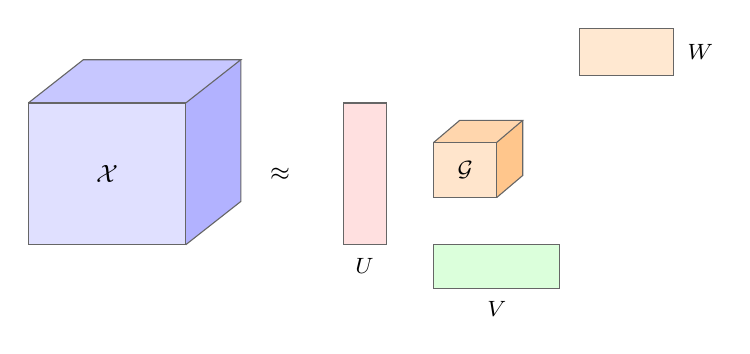
\begin{tikzpicture}[x=1cm,y=1cm,font=\small,>=stealth]
  \fill[blue!12] (0,0) -- (2.0,0) -- (2.0,-1.8) -- (0,-1.8) -- cycle;
  \fill[blue!22] (0,0) -- (2.0,0) -- (2.7,0.55) -- (0.7,0.55) -- cycle;
  \fill[blue!30] (2.0,0) -- (2.7,0.55) -- (2.7,-1.25) -- (2.0,-1.8) -- cycle;
  \draw[black!60] (0,0) -- (2.0,0) -- (2.0,-1.8) -- (0,-1.8) -- cycle;
  \draw[black!60] (0,0) -- (0.7,0.55) -- (2.7,0.55) -- (2.0,0);
  \draw[black!60] (2.7,0.55) -- (2.7,-1.25) -- (2.0,-1.8);
  \node at (1.0,-0.9) {\(\mathcal X\)};
  \node at (3.2,-0.9) {\(\approx\)};
  \begin{scope}[shift={(4.0,0)}]
    \draw[black!60,fill=red!12] (0,0) rectangle (0.55,-1.8);
    \node[below,font=\footnotesize] at (0.27,-1.85) {\(U\)};
    \fill[orange!20] (1.15,-0.5) -- (1.95,-0.5) -- (1.95,-1.2) -- (1.15,-1.2) -- cycle;
    \fill[orange!32] (1.15,-0.5) -- (1.95,-0.5) -- (2.28,-0.22) -- (1.48,-0.22) -- cycle;
    \fill[orange!45] (1.95,-0.5) -- (2.28,-0.22) -- (2.28,-0.92) -- (1.95,-1.2) -- cycle;
    \draw[black!60] (1.15,-0.5) -- (1.95,-0.5) -- (1.95,-1.2) -- (1.15,-1.2) -- cycle;
    \draw[black!60] (1.15,-0.5) -- (1.48,-0.22) -- (2.28,-0.22) -- (1.95,-0.5);
    \draw[black!60] (2.28,-0.22) -- (2.28,-0.92) -- (1.95,-1.2);
    \node[font=\footnotesize] at (1.55,-0.85) {\(\mathcal G\)};
    \draw[black!60,fill=green!14] (1.15,-2.35) rectangle (2.75,-1.8);
    \node[below,font=\footnotesize] at (1.95,-2.4) {\(V\)};
    \draw[black!60,fill=orange!18] (3.0,0.35) rectangle (4.2,0.95);
    \node[right,font=\footnotesize] at (4.25,0.65) {\(W\)};
  \end{scope}
\end{tikzpicture}

\emph{把上一节换基图里的三个方阵换成瘦长的矩阵，中间的核心随之缩小。\(U,V,W\) 各挑出一个模上的低维子空间，\(\mathcal G\) 记录这些方向之间怎样组合。CP 只允许第 \(r\) 个用户因子配第 \(r\) 个商品、时间因子，Tucker 核则允许第 \(p\) 个用户方向与第 \(q\) 个商品方向、第 \(r\) 个时间方向任意搭配。}
\end{center}

参数量约为 \(Ir_1+Jr_2+Kr_3+r_1r_2r_3\)，核心那一项会随三个秩相乘膨胀，所以 Tucker 适合每个模都确有低维结构的场合。哪个模压不动，对应的 \(r_k\) 就不该硬压。

秩的形态也跟着变。把三阶张量沿各模展开得到 \(X_{(1)},X_{(2)},X_{(3)}\)，多线性秩定义为

\[
\bigl(\rank X_{(1)},\ \rank X_{(2)},\ \rank X_{(3)}\bigr),
\]

三个数分别衡量每个模需要多少独立方向。它们互相不必相等，也不等于 CP 秩。矩阵的秩是一个数，三阶的秩变成一个元组——Tucker 的目标秩 \((r_1,r_2,r_3)\) 正是在分别控制三个展开矩阵的列空间维数。到这里已经有四个不同的对象了：阶、各模维度、CP 秩、多线性秩。

\subsection{Tucker 这边保证还在，只是弱了一档}

高阶 SVD（HOSVD）的构造是个骨架：对每个展开矩阵 \(X_{(k)}\) 做一次 SVD，取前 \(r_k\) 个左奇异向量当作该模的因子，再把原张量沿三个模投影回这些子空间得到核心 \(\mathcal G=\mathcal X\times_1U^{\trans}\times_2V^{\trans}\times_3W^{\trans}\)，重构就是 \(\mathcal G\times_1U\times_2V\times_3W\)。

它像 SVD，但核心不是超对角的。矩阵 SVD 里只有同编号的左右奇异向量通过 \(\Sigma\) 配对；Tucker 核保留了跨编号的交互，非对角元素一般不为零。

好消息在于，多线性秩不超过 \((r_1,r_2,r_3)\) 的张量集合是闭的，最佳近似确实存在。截断 HOSVD 未必是那个最佳者，但它满足一个准最优界：对 \(N\) 阶张量，它的误差不超过最优误差的 \(\sqrt{N}\) 倍，三阶就是 \(\sqrt{3}\)。有了这个界，一次闭式计算就能拿到一个误差可控的起点；高阶正交迭代在此基础上交替改进各模子空间，通常更好，但仍可能停在局部最优。

把两边并排看：CP 的目标可能无人达到，Tucker 的目标存在且有一个便宜的准最优近似。选分解时这一条常常比参数量更重要。

\subsection{两种分解在问不同的问题}

CP 假设数据由少数跨所有模一一配对的可分离机制叠加而成，核心相当于只有超对角非零。参数少，成分读起来直接，麻烦在于秩的选择缺乏可靠准则、优化脆弱、退化风险实打实。Tucker 假设每个模各自落在一个低维子空间，核心承载丰富交互，更接近多模版本的 PCA；它更灵活也更稳，欠下的是核心的旋转不唯一（往因子里插一个正交矩阵、往核心里插它的转置，重构不变）和更多参数。

矩阵 SVD 同时占了两边的便宜：秩一配对、正交子空间、对角核心、最佳截断、唯一的奇异值序列，这些性质在二阶恰好合流成一件事。它们在三阶各自散开，而不是一起消失——CP 丢的是最优性与正交性，Tucker 丢的是唯一性与超对角形式。

两者也能串起来用：把 Tucker 核限制成只有 \(g_{rrr}\) 非零就退回 CP 形式；先用 Tucker 把大张量压成小核心，再对核心做 CP，是常见的省时做法。选哪个，取决于你更相信``存在少数可分离机制''还是``每个模有低维子空间及其交互''，名字本身没有高下。

\subsection{分解之前的那些决定}

以上都默认所有条目彼此可比，误差用 Frobenius 范数度量。这个默认经常不成立。计数数据用 Poisson 损失更合适，二元事件用 Bernoulli；缺失条目不能填零后当作已观测，正确做法是只在观测集合上算损失。需要可解释的加性部件时可以给因子加非负约束，但这一步会让 HOSVD 的闭式计算和误差保证同时失效，只能回到迭代求解。

各模的尺度会悄悄支配结果。某些时段观测更密、某类用户的数值天然更大，平方误差就优先服务这些高权重区域。中心化在张量里也不再只有一种做法：可以减全局均值，也可以分别移除用户、商品或时间的主效应，减掉的东西不同，剩下的``结构''就不同。预处理等于在声明哪些变化算信号、哪些算基线。

最后一句留给结果的读法。重构误差低不自动带来可解释的因子，也不自动带来下游预测的提升。CP 与 Tucker 找到的是在你所选损失和约束下的多线性结构，因果、业务语义和外推稳定性需要另外的证据。回到开头那两次对不上的运行：现在它不再是可疑现象，而是一份诊断——若换个初始化因子就变样，说明数据没能把成分钉住，此时该问的是唯一性条件是否满足、\(R\) 是否取大了，而不是挑一份看着顺眼的结果报出去。什么时候回来翻这一节？当你看到成分范数持续增大而误差只肯缓慢下降的时候。
